
\chapter{Methodology}\label{chap:related_works}


\section{Configuration}\label{sec:2-spec}
In this experimental setup, two fundamental sensors are employed to acquire and analyze data.
The Realsense D435i camera, 
known for its high-resolution image capture and depth-sensing capabilities, is utilized for visual data acquisition. 
Complementing the camera is the AWR1843boost mmWave radar, operating in the 77-81GHz frequency range. 
Both sensors are securely housed within a custom 3D-printed enclosure as seen in figure \ref{fig:radar_camera_setup_fig}, 
which not only safeguards them but also minimizes external interference, ensuring the integrity of data acquisition. 
The mmWave radar config that is used is a 77-81GHz chirp, with settings balanced between range and resolution,
collecting data at 20 frames per second.

\begin{figure}[hpbt]
    \centering
    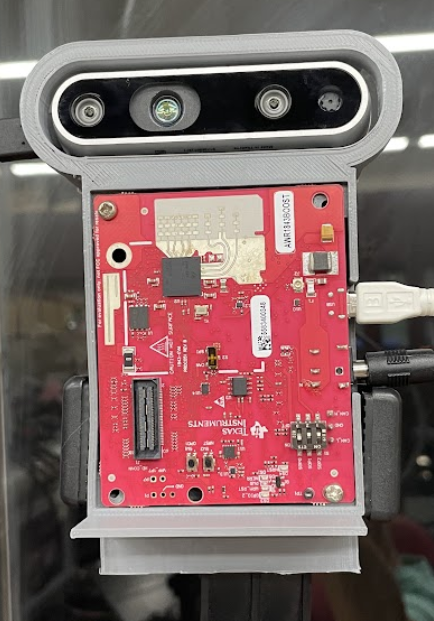
\includegraphics[width=5cm]{Figures/radar_camera_setup.png}%\textwidth
    \caption{Radar camera setup}
    \label{fig:radar_camera_setup_fig}
\end{figure}


\section{Overview}\label{sec:2-overview}
Overview block diagram of the algorithm shown in figure \ref*{fig:kf_update}.
\begin{figure}[hpbt]
    \centering
    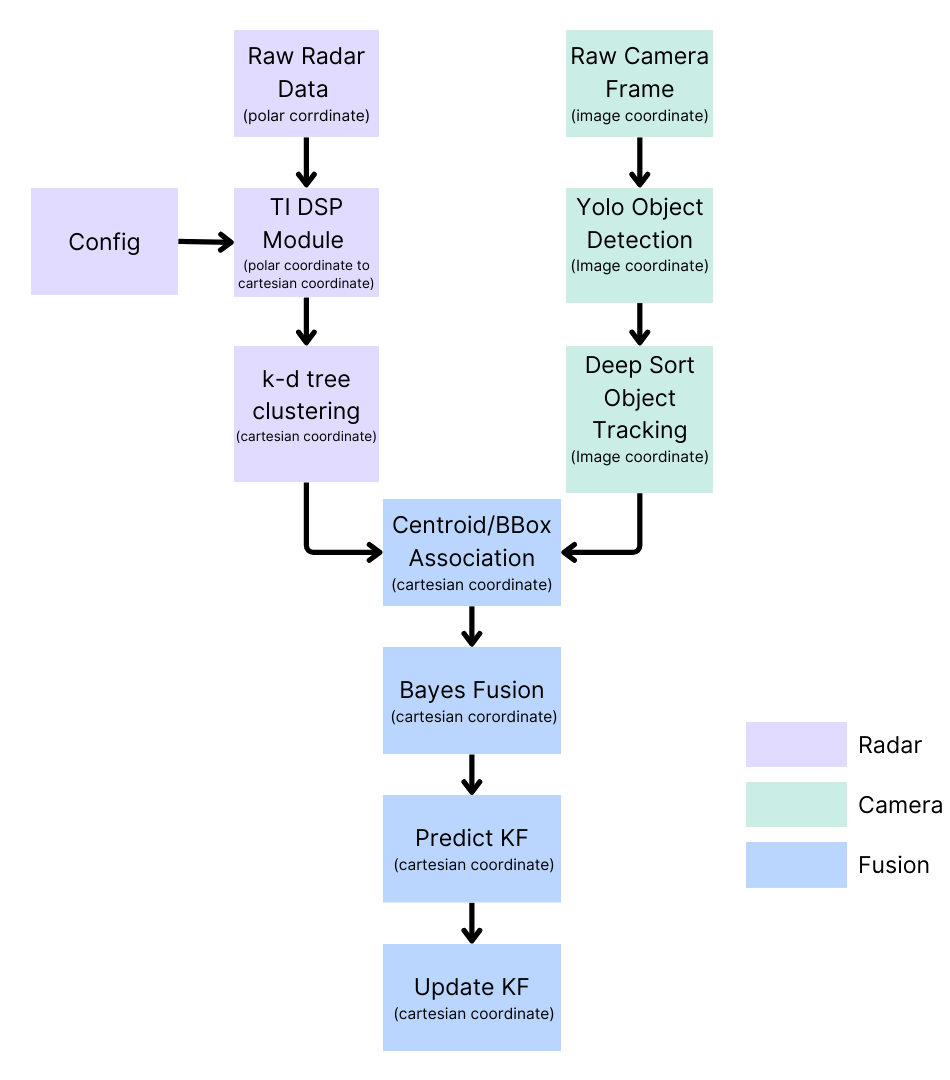
\includegraphics[width=10cm]{Figures/kf_update-modified.png}%\textwidth
    \caption{Radar camera Kalman Filter workflow}
    \label{fig:kf_update}
\end{figure}

\section{Calibration}\label{sec:2-calibration}
\subsection{Camera Calibration}
To accurately map the monocular camera's image coordinates to real-world coordinates, calibration of intrinsic and extrinsic is required.
Using tools provided by ROS \cite{cam_calib} as shown in figure \ref*{fig:camera_calibration}.

\begin{figure}[hpbt]
    \centering
    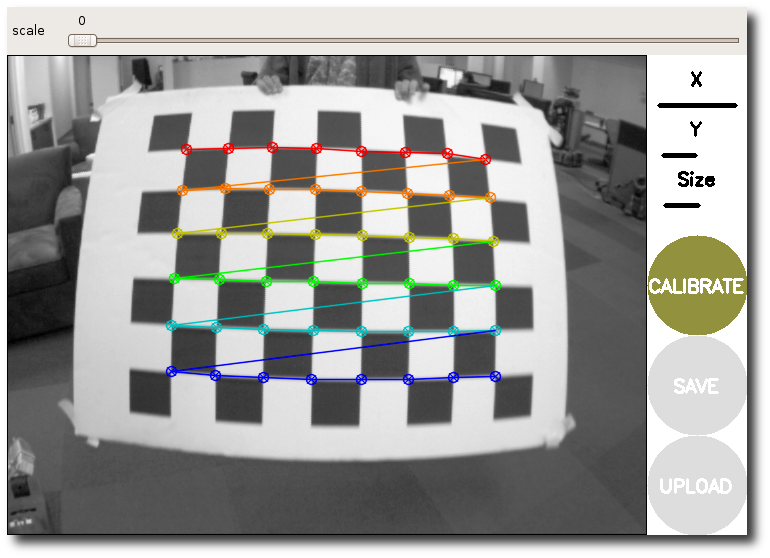
\includegraphics[width=8cm]{Figures/cam_calib.png}%\textwidth
    \caption{Camera extrinsic and intrinsic calibration}
    \label{fig:camera_calibration}
\end{figure}

\subsection{Radar-Camera Calibration}
In order to achieve accurate sensor fusion, it is essential to conduct proper calibration of the two sensors. 
For this purpose, a corner reflector is employed (figure \ref*{fig:radar_camera_calibration} \subref{subfig:corner_reflector_fig}), primarily due to its strong radar reflection characteristics(white point in figure \ref*{fig:radar_camera_calibration} \subref{subfig:radar_view_fig}). 
Additionally, it offers the advantage of appearing as a single point in both radar and camera data, effectively reducing ambiguity (figure \ref*{fig:radar_camera_calibration} \subref{subfig:camera_view_fig}).

Data points from both radar and camera coordinates can be collected with the corner reflector positioned at various locations.
After data is collected, radar points are associated with image points based on equation \ref*{equ:img2cart}
\begin{figure}[hbpt]
    \centering
    \begin{subfigure}{0.25\linewidth}
        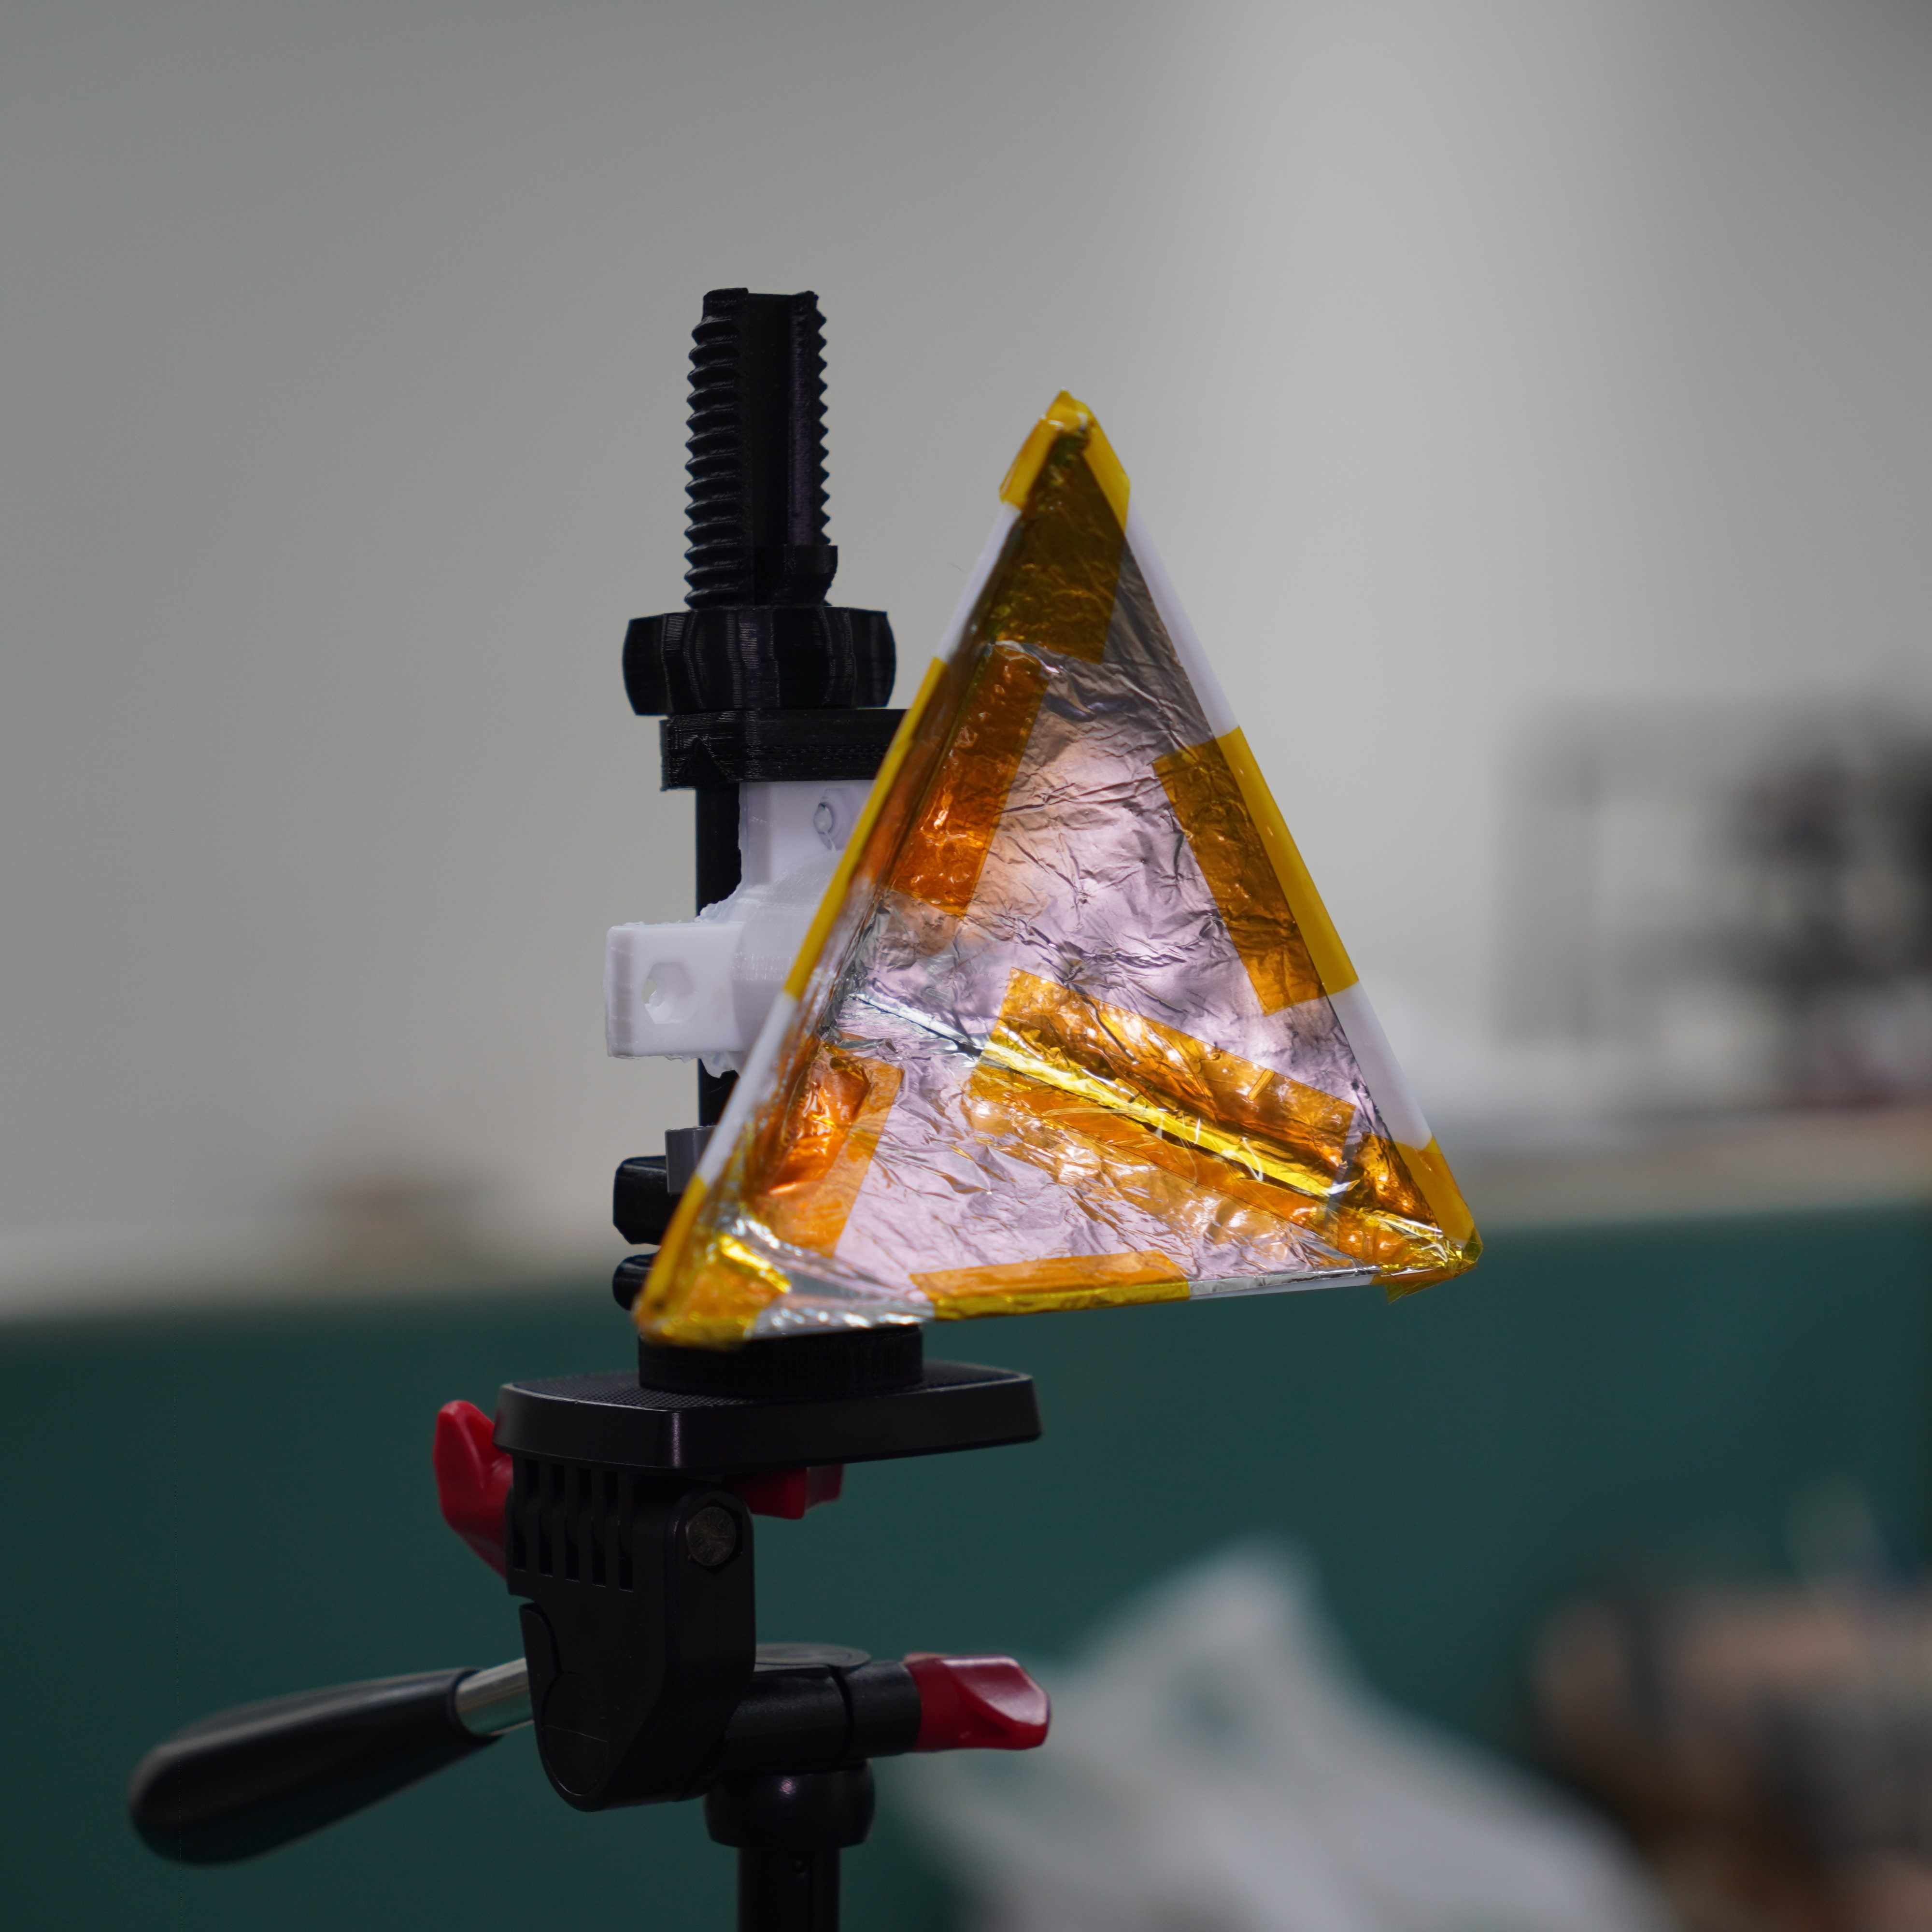
\includegraphics[width=5.5cm]{Figures/corner_reflector.jpg}
        \caption{Radar Corner Reflector}
        \label{subfig:corner_reflector_fig}
    \end{subfigure}
    \hfill
    \begin{subfigure}{0.25\linewidth}
        \centering
        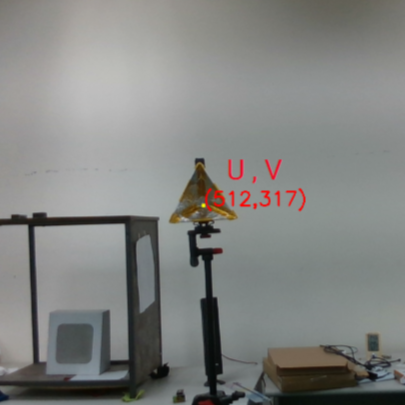
\includegraphics[width=5.5cm]{Figures/camera_corner.png}
        \caption{Camera-corner reflector calibration}
        \label{subfig:camera_view_fig}
    \end{subfigure}
    \hfill
    \begin{subfigure}{0.25\linewidth}
        \centering
        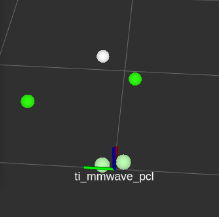
\includegraphics[width=5.5cm]{Figures/radar_corner.png}
        \caption{Radar-corner reflector calibration}
        \label{subfig:radar_view_fig}
    \end{subfigure}

    \caption{Radar camera calibration}
    \label{fig:radar_camera_calibration}
\end{figure}

\section{Data Pre-Processing}\label{sec:2-preprocessing}
\subsection{mmWave Radar Data Pre-Processing}\label{sec:2-kd_tree}
Given that radar data is inherently sparse and noisy, its data needed to be filtered.
For this purpose, k-d tree is employed to cluster the pointcloud.
A k-d tree, short for k-dimensional tree, is a hierarchical data structure used for efficient multidimensional data organization and search operations. 
It arranges data points in k-dimensional space, such as spatial coordinates, in a binary tree structure. 

\subsection{Image Recognition and Tracking\small(to be done)}\label{sec:2-img_recognition}
yolov3 \cite{redmon2018yolov3} and deepsort \cite{Wojke2017simple}.

Before fusing, the detection results need to be converted into cartesian coordinates.

Conversion image to real-world vector, seen in figure \ref{fig:camera_projection}.
\begin{equation}\label{equ:img2cart}
u=c_x-\frac{p_x}{p_y}f
\end{equation}
where
\begin{align*}
    c_x &=\text{center of camera image in pixel}\\
    p_x &=\text{x-axis position in cartesian}\\
    p_y &=\text{y-axis position in cartesian}\\
    f &=\text{camera focal length in pixel}\\
    u &=\text{center of Bbox object detection in pixel}
\end{align*}

From equation \ref{equ:img2cart} we can obtain
\begin{equation}\label{equ:2_img2cart2}
    u=640-\frac{p_x}{p_y}950
\end{equation}

Thus
\begin{equation}\label{equ:2_cam_px}
    p_{x_{cam}}=
    \frac
    {(640-u)p_{y_{radar}}}
    {950}
\end{equation}






\begin{figure}[hpbt]
    \centering
    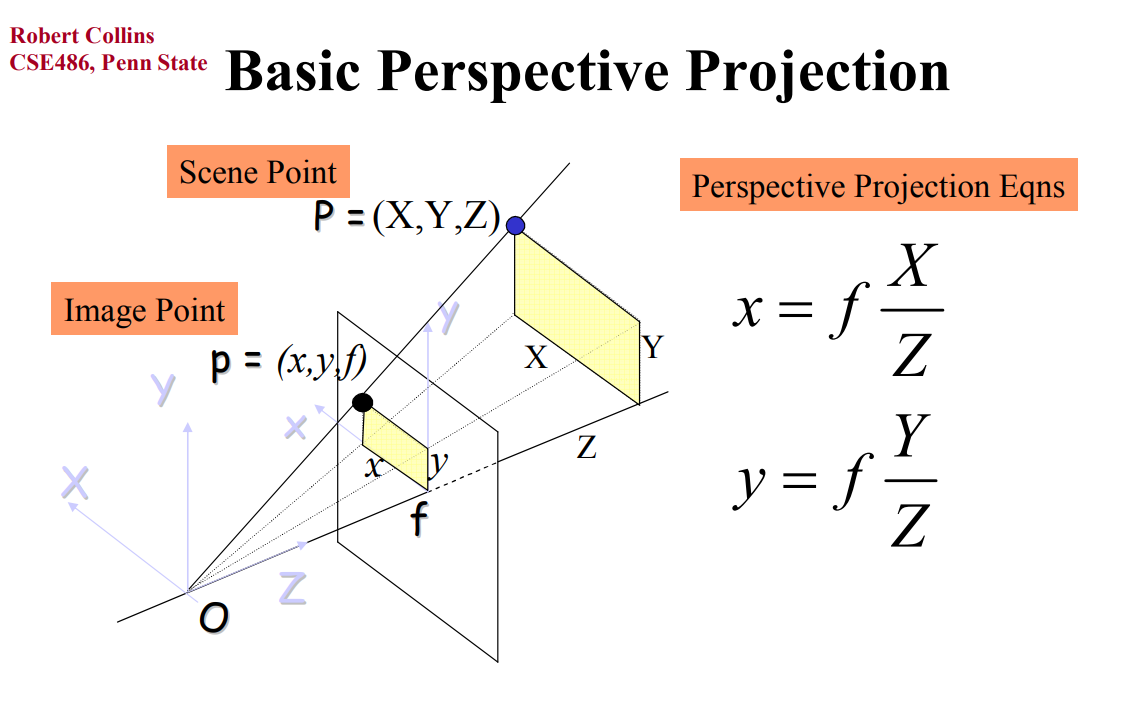
\includegraphics[width=8cm]{Figures/cam_projection.png}%\textwidth
    \caption{Camera to real-world projection}
    \label{fig:camera_projection}
\end{figure}

\section{Radar-camera Data Association}\label{sec:2-association}
Before fusion, radar clusters have to be associated with tracked objects from deepsort.
First, centroids of radar clusters are mapped into image coordinates.
Second, is to find the theoretical error of radar's measurement \cite{8844649}, which is radar's resolution, determined by equation \ref*{equ:angular_resolution}
Finally, if the distance between the calculated radar centroid and the image detection lies within the theoretical boundary
, we can safely assume both measurements belong to the same object of interest.
\begin{equation}\label{equ:angular_resolution}
    \Delta \theta= \frac{c_0}{f_c d N_{RX} N_{TX} \cos(\theta _i)}
\end{equation}
where
\begin{align*}
    f_c & = \text{center frequency} \\
    \lambda & = \text{carrier signal wavelength} \\
    d & =  \lambda/2 \\
    N_{RX} & = \text{Number of receiving antenna}\\
    N_{TX}& = \text{Number of transferring antenna}\\
    \theta _i &= \text{angle of interest}
\end{align*}

\section{Bayes Fusion}\label{sec:2-bayes_fusion}

The coordinates that undergo fusion from both radar and image sensors are the horizontal coordinates,
specifically the radar's azimuth and the image's "u" coordinate. 
This constraint arises from the fact that these are the only coordinates where both sensors provide measurements, 
as illustrated in Figure \ref{fig:trade_off_and_plane}\subref{subfig:cam_radar_sub}.
It's important to note that radar's elevation measurement resolution is limited and subject to noise. 
Additionally, the image sensor does not provide depth information.

If X is the real position of the object, 
then Bayes' theorem predicts that the probability of the fused position is shown in equation \ref{equ:bayes1} \cite{10.1007/978-981-16-2248-9_32}.

\begin{equation}\label{equ:bayes1}
    P_{prob}(\frac{P}{X})=
    \frac
    {e \frac{−(P−X)^T R^{−1}(P−X)}{2}}
    {2 \pi R^(0.5)}
\end{equation}

Applying Bayes' fusion, the value of the measured measurements is provided by equation \ref{equ:bayes2}.

\begingroup
\Large
\begin{equation}\label{equ:bayes2}
P_{x_{bayes}}=\frac
{\frac{p_{x_{radar}}}{R_{radar}}+\frac{p_{x_{cam}}} {R_{cam}}}
{\frac{1}{R_{radar}}+\frac{1}{R_{cam}}}
\end{equation}
\endgroup

where
\begin{align*}
    P_{x_{bayes}} &= \text{fused position}\\
    p_{x_{radar}} &= \text{radar x-axis in cartesian}\\
    p_{x_{cam}} &= \text{camera x-axis in cartesian}\\
    R_{radar} &= \text{radar covariance}\\
    R_{cam} &= \text{camera covariance}
\end{align*}
\begin{equation}\label{equ:bayes4}
    \frac{1}{R}=\frac{1}{R_1}+\frac{1}{R_2}
\end{equation}
\begin{equation}\label{equ:2-radar_R}
    \mathbf{R}_{radar} = 
        \sigma_{radar_x}^2 
\end{equation}
\begin{equation}\label{equ:2-R_cam}
    \mathbf{R}_{cam} = 
        \sigma_{cam_u}^2
\end{equation}


\section{Multimodal Kalman Filter}\label{sec:2-kalman_filter}
\subsection{Predict}\label{sec:2-predict}
The state matrix used in this Kalman Filter is from the single sensor maneuvering tracking, with constant velocity.
It has four elements and is defined with position and velocity, which projects onto the x-axis and y-axis:

\begin{equation}\label{equ:state_eq}
    \mathbf{x} = 
        \begin{bmatrix} 
        p \\ 
        v 
        \end{bmatrix} = 
        \begin{bmatrix} 
        P_{x_{bayes}} \\ 
        p_y \\ 
        v_x \\ 
        v_y 
        \end{bmatrix}
\end{equation}
where
\begin{align*}
    P_{x_{bayes}} &=\text{Bayes fusion position x}\\
    p_y &=\text{position y}\\
    v_x &=\text{velocity x}\\
    v_y &=\text{velocity y}\\
\end{align*}

\begin{equation}\label{equ:transition_matrix_H}
    \mathbf{F} = 
    \begin{bmatrix}
        1 & 0 & 1 & 0 \\
        0 & 1 & 0 & 1 \\
        0 & 0 & 0 & 0 \\
        0 & 0 & 0 & 0 \\
      \end{bmatrix}
\end{equation}

\begin{equation}\label{equ:predict_eq}
    \mathbf{x}_k=\mathbf{F}_k\mathbf{x}_{k-1}+\mathbf{w}
\end{equation}

Error covariance update
\begin{equation}\label{equ:error_covariance}
    \mathbf{P}_k=\mathbf{F}_k \mathbf{P}_{k-1} \mathbf{F}_k^T+\mathbf{Q}_k
\end{equation}

\subsection{Update}\label{equ:2_update}
To fuse two sensors with different update rates, Kalman Filter is updated seperately (figure \ref{fig:sync_fig})
\begin{figure}[hpbt]
    \centering
    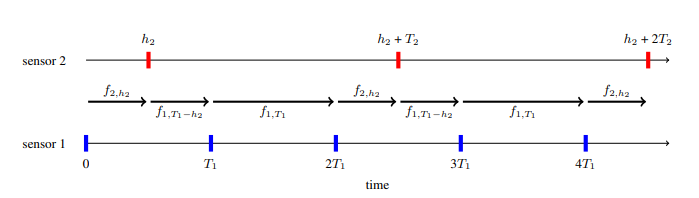
\includegraphics[width=\textwidth]{Figures/sync.png}%\textwidth
    \caption{Update timing \cite{7472511}}
    \label{fig:sync_fig}
\end{figure}
\newpage
\subsubsection{Radar Update}\label{sec:2-radar_update}  
Centroid of radar
\begin{equation}
    \mathbf{z}_{radar}=
    \begin{bmatrix}
        P_{x_{bayes}} \\ 
        p_y
    \end{bmatrix}
\end{equation}
\begin{equation}\label{equ:2_radar_R_kf}
    \mathbf{R}_{radar} = 
    \begin{bmatrix}
        \sigma_{radar_x}^2 & 0 \\
        0 & \sigma_{radar_y}^2 \\
      \end{bmatrix}
\end{equation}
Transition matrix
\begin{equation}\label{equ:2_radar_transition_matrix}
    \mathbf{H} = 
    \begin{bmatrix}
        1 & 0 & 0 & 0 \\
        0 & 1 & 0 & 0 \\
      \end{bmatrix}
\end{equation}



\subsubsection{Camera Update}\label{sec:2-camera_update}
\begin{equation}\label{equ:2_z_cam}
    \mathbf{z}_{cam}=
    \begin{bmatrix}P_{x_{bayes}}\end{bmatrix}
\end{equation}

\begin{equation}\label{equ:2_cam_transition_matrix}
    \mathbf{H} = 
    \begin{bmatrix}
        1 & 0 & 0 & 0 \\
      \end{bmatrix}
\end{equation}

